\newcommand{\yandex}{\mbox{<<Яндекс>>}}
\newcommand{\yandexbel}{\mbox{<<ЯндексБел>>}}
\newcommand{\rubinplaza}{\mbox{Рубин Плаза}}

\section[Обеспечение пожарной безопасности на предприятии]{Обеспечение пожарной безопасности на предприятии \yandexbel{}}

Целью дипломного проектирования явилась разработка программного средства для обнаружения радиосигналов с помощью SDR-приемника. С его помощью можно сканировать радиоэфир, выделяя наиболее сильные источники сигнала, а также исследовать отдельные частоты, определяя нешумовые последовательности. Аппаратная часть проекта обеспечена приемником на базе software defined radio, что позволяет значительно сократить материальные расходы в сравнении с традиционными системами. В настоящем разделе рассмотрим вопросы, связанные с обеспечением пожарной безопасности в компании \yandexbel{}.

Разработка выполнялась при прохождении преддипломной практики в компании \yandexbel{}. \yandexbel{} --- дочерняя компания \yandex{}. Основным направлением ее деятельности является разработка программного обеспечения. Белорусскому офису всего несколько лет, но сейчас там работает более ста человек и ожидается дальнейший рост. Офис располагается в двух блоках бизнес-центра \rubinplaza{}.

\rubinplaza --- современный бизнес-центр категории Б. Помимо \yandexbel{} в нем работают команды EPAM Systems, Onliner, БПС-Сбербанк. Планировка здания обеспечивает высокий уровень пожарной безопасности. Каждый офисный блок имеет два выхода. Парадный выход оборудован лифтами и лестницей, пожарный --- только лестницей. На каждом этаже имеется свободный доступ к им обоим. Огнезащитное покрытие конструкций изолирует секции этажа, предотвращая распространение пламени.

Въезд на территорию бизнес-центра контроллируеся охраной. Блокирование проездов и проходов не допускается. Внешняя сторона здания остеклена, что позволяет использовать оконные проемы для экстренного доступа в помещения.

Для отопления помещений используются приборы центрального водяного отопления. Воздухонагревательные приборы объединены в вентиляционную систему здания. Воздуховоды вмонтированы в межэтажные перекрытия и недоступны извне. Электросеть здания также проложена в межсекционных перегородках и межэтажных перекрытиях. Для подключения к ней в стены встроены розетки. Работники компании подключаются к электросети через сетевые фильры, защищающие от резких скачков напряжения. В помещениях имеется достаточное количество розеток для подключения всего необходимого электрооборудования сотрудников.

За пожарную безопасность в \yandexbel{} отвечает директор компании. После найма сотрудники проходят инструктаж по установленному противопожарному режиму и мерам безопасности при работе с электрооборудованием. Курение внутри здания запрещено, в каждом помещении установлены пожарные извещатели. Рабочие места организованы таким образом, чтобы организовать беспрепятственный доступ к сетевым фильтрам и проложить кабели электроприборов вне рабочей области людей.

В коридорах установлены пожарные краны (рисунок \ref{fig:fireplug}). Ключи к ним находятся в специальных застекленных отсеках и в случае экстренной ситуации могут быть быстро извлечены без посторонней помощи. Пожарные краны сгруппированы в блоки примерно по 2 крана на кабинет.

\begin{figure}[H]
  \begin{center}
    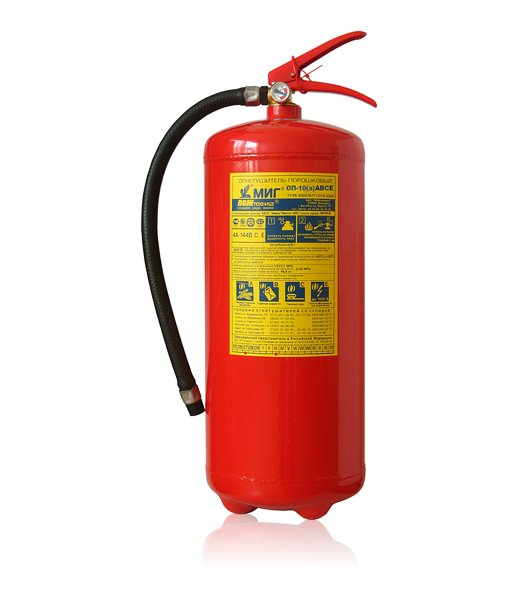
\includegraphics[height=0.4\textheight]{extinguisher}
    \caption{Порошковый огнетушитель \mbox{ОП-10} (з) МИГ М}
    \label{fig:extinguisher}

    \vspace{0.05\textheight}

    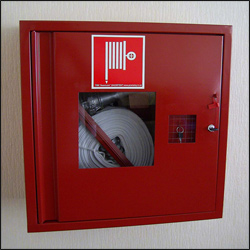
\includegraphics[height=0.4\textheight]{fireplug}
    \caption{Пожарный кран}
    \label{fig:fireplug}
  \end{center}
\end{figure}

Для оперативного тушения пламени в кабинетах установлены порошковые огнетушители (рисунок \ref{fig:extinguisher}) и оросительная система пожаротушения.

Каждый кабинет оборудован пожарными дымовыми оптико-электронными точечными извещателями \mbox{ИП212-02М1} (рисунок \ref{fig:auto_fire_detector}). Дымовые извещатели работают по принципу контроля оптических свойств окружающей среды. Они обнаруживают возгорание по изменению светового потока, то есть прозрачности воздуха или по яркости отраженного света от частиц дыма. Оптико-электронные датчики легко фиксируют дым серого цвета, образующийся на начальной стадии тления. В коридорах дополнительно установлены ручные пожарные извещатели \mbox{ИП 5-2Р} (рисунок \ref{fig:manual_fire_detector}). С их помощью человек, обнаруживший признаки возгорания, может подать сигнал о пожаре не дожидаясь срабатывания автоматических средств.

Таким образом, изложенные выше предложения обеспечивают пожарную безопасность в компании \yandexbel{}.

\begin{figure}
  \begin{center}
    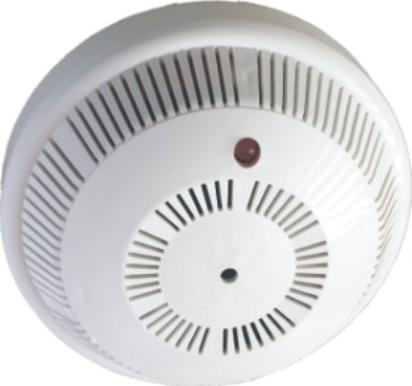
\includegraphics[height=0.4\textheight]{auto_fire_detector}
    \caption{Автономный пожарный извещатель}
    \label{fig:auto_fire_detector}

    \vspace{0.05\textheight}

    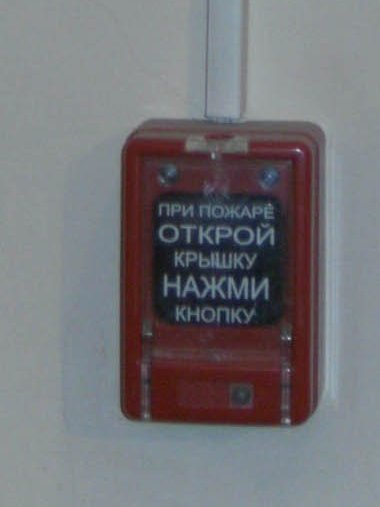
\includegraphics[height=0.4\textheight]{manual_fire_detector}
    \caption{Ручной пожарный извещатель}
    \label{fig:manual_fire_detector}
  \end{center}
\end{figure}
